\documentclass[a4paper]{report}

\usepackage{../mathstemplate}

\date{IV семестр, весна 2024 г.}
\title{Дифференицальная геометрия. Неофициальный конспект}
\author{Лектор: Нина Дмитриевна Лебедева \\ Конспектировал Леонид Данилевич}

\begin{document}
    \shorthandoff{"}
    \maketitle
    \tableofcontents
    \newpage
    \setcounter{lection}{0}


    \chapter{Риманова геометрия}
    \newlection{14 февраля 2024 г.}
\section{Гладкие многообразия}
    \definition[Топологическое многообразие]{
        Хаусдорфово топологическое пространство $M$ со счётной базой, такое что $\forall x \in M: \exists U \ni x: U \sim \R^n$.
        Данное число $n$ называется \emph{размерностью} многообразия, пишут $\dim M = n$, или часто пишут это число верхним индексом: $M^n$.
    }
    Далее пусть $M^n$ --- топологическое многообразие.
    \definition[Карта]{
        Пара из открытого $U \subset M^n$, и гомеоморфизма $\phi: U \map \Omega$, где открытое $\Omega \subset \R^n$.
    $U$ называется \emph{носителем карты}.
    }
    <<В половине случаев в литературе картой называется обратное отображение>>.
    \definition[Атлас]{
    Набор карт $(U_i, \phi_i)$, таких, что $\bigcup\limits_{i}U_i = M$.
    }
    Пусть даны две карты $(U, \phi)$ и $(V, \psi)$.
    Далее удобно считать, что их носители пересекаются: $U \cap V \ne \o$, иначе определение не несёт смысла.
    \definition[Отображение перехода]{
    Отображение $\psi \circ \phi^{-1}: \phi(U \cap V) \map \psi(U \cap V)$. Обозначается $f_{\phi\psi}$
    }
    \definition[Карты $(U, \phi)$ и $(V, \psi)$ согласованы]{
        Отображение перехода и ему обратное гладкие.
    }
    \definition[Гладкий атлас]{
    Атлас, такой, что любые две карты согласованы.
    }
    Далее все атласы предполагаются гладкими.
    \definition[Атласы эквивалентны]{
        Их объединение (то есть все карты из первого и из второго атласа вместе взятые) --- тоже гладкий атлас.
    }
    \proposal{
    Эквивалентность атласов --- отношение эквивалентности.
    }
    \definition[Гладкая структура на многообразии]{
    Максимальный гладкий атлас (атлас, к которому нельзя добавить карт).
    }
    \note{
        К атласу можно добавить произвольное количество карт, согласованных с теми, что в атласе, и они будут согласованы между собой.
    В частности, для задания гладкой структуры достаточно произвольного атласа $A$: в $A$ можно добавить всевозможные карты, согласованные с картами из $A$, и он станет максимальным.
    }
    \definition[Гладкое многообразие]{
    Многообразие с гладкой структурой.
    }
    \examples[Атласы]{
    \item Стандартная гладкая структура на $\R^n$ задаётся атласом $\{(\R^n, \id)\}$.
        \item В частности, стандартная структура на $\R^1$ задаётся атласом $\{(\R^1, [x \mapsto x])\}$.
    \item Можно задать нестандартную структуру на $\R^1$: $\{(\R^1, [x \mapsto x^3])\}$.
    \precaution{
        Это действительно гладкая структура, хотя обратное отображение ${[x \mapsto x^{\nicefrac{1}{3}}]}$ не гладкое.
        Тем не менее, определение и не требует гладкости от него.
    }
    \item Пусть $f = \all{x, & x \ge 0 \\ \frac{1}{2}x,&x \le 0}$. Тогда $\{(\R^1, f)\}$ --- тоже гладкий атлас на $\R^1$.

    Тем не менее, любые два атласа из приведённых выше атласов на $\R^1$ не эквивалентны --- отображения перехода получаются не гладкими.
    \item Гладкая структура на сфере задаётся двумя картами: пусть $S^2$ --- сфера с северным полюсом $N$ и южным $S$, пусть $f, g$ --- стереографические проекции с данными полюсами.
        Тогда ${\{(S^2 \sm \{N\}, f), (S^2 \sm \{S\}, g)\}}$ --- атлас.
    }
    \note{
    Если $M$ --- гладкое многообразие, и открытое $W \subset M$, то на $W$ естественным образом определена гладкая структура, наследующаяся с $M$.
    }
    \subsection{Гладкие отображения}

    Пусть $M^m, N^n$ --- гладкие многообразия, $A_M, A_N$ --- соответствующие атласы.
    Рассмотрим отображение $f: M \map N$.
    \definition[Координатное представление $f$ в картах $(U, \phi)$ на $M$ и $(V, \psi)$ на $N$]{
        Такое $\tilde{f}: \phi(U) \map \psi(V)$, что диаграмма коммутативна везде, где определена (то есть $\tilde{f} = \psi \circ f \circ \phi^{-1}$ на $\phi(U \cap f^{-1}(V))$).
        % https://q.uiver.app/#q=WzAsNCxbMCwxLCJcXHBoaShVKSJdLFsxLDEsIlxccHNpKFYpIl0sWzAsMCwiVSJdLFsxLDAsIlYiXSxbMiwwLCJcXHBoaSJdLFszLDEsIlxccHNpIl0sWzIsMywiZiJdLFswLDEsIlxcdGlsZGV7Zn0iXV0=
        \[\begin{tikzcd}[ampersand replacement=\&]
              U \& V \\
              {\phi(U)} \& {\psi(V)}
              \arrow["\phi", from=1-1, to=2-1]
              \arrow["\psi", from=1-2, to=2-2]
              \arrow["f", from=1-1, to=1-2]
              \arrow["{\tilde{f}}", from=2-1, to=2-2]
        \end{tikzcd}\]
    }
    Далее считаем, что $f: M \map N$ непрерывна (эквивалентно, все координатные представления непрерывны).
    \definition[$f$ гладкое]{
    Любое координатное представление --- гладкое.
    }
    \definition[$f$ --- гладкое в точке $x \in M$]{
    Найдётся окрестность $U_x \ni x$ и карты $(U, \phi)$, $(V, \psi)$ (где $V \ni y \coloneqq f(x)$), такие, что $U_x \subset U$ и сужение на $U_x$ координатного представления $f$ --- гладко.
    }
    \properties[Гладкие отображения]{
    \item Гладкость в точке не зависит от выбора карт.
    \item Гладкость отображения не зависит от выбора атласа в одном классе эквивалентности.
    \item Отображение гладкое $\iff$ оно гладкое в любой точке. \comment{На лекции было доказательство $\when$.}
    \item Пусть $f: M \map N, g: N \map K$ гладкие. Тогда их композиция $g \circ f$ гладкая.
    \item Тождественное отображение гладкое, если в образе и прообразе выбраны эквивалентные атласы.
    \item Определение гладкости отображения совпадает с определением гладкости из матанализа (если считать, что $M \subset \R^n$ открыто, и порождающий атлас состоит из тождественной карты)
    }
    \definition[Диффеоморфизм $f: M \map N$]{
    Гладкое $f$, такое, что $f^{-1}$ --- тоже гладкое.
    }
    \definition[Многообразия $M$ и $N$ диффеоморфны]{
    Между ними существует диффеоморфизм.
    }
    Понятно, что диффеоморфность --- отношение эквивалентности.
    \statement{
    Если $M^m \overset{\text{диф}}\sim N^n$, то $m = n$.
    \provehere{
    Рассмотрим произвольную $x \in M$.
    Пусть $f: M \map N$ --- диффеоморфизм, пусть $\tilde{f}$ --- его координатное представление.
        Тогда $\tilde{f}^{-1}$ --- координатное представление $f^{-1}$, откуда $\tilde{f}^{-1}$ --- тоже гладкое.
     Рассмотрим дифференциал $\d_x{\tilde{f}}(\_)$, это изоморфизм векторных пространств, значит, $m = n$.
    }
    }
    По умолчанию всегда считается, что на $\R^m$ введена стандартная гладкая структура.
    \proposal{
        Пусть $M$ --- гладкое многообразие, тогда карта --- диффеоморфизм между $U$ и $\phi(U)$.
        Обратно, любой диффеоморфизм между открытым подмножеством $W \subset M$ и областью $\Omega \subset \R^m$ --- карта.
        \provehere{
        \[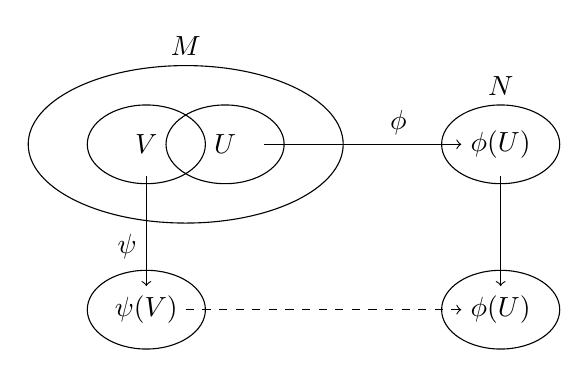
\begin{tikzpicture}
              \draw (-2,2) ellipse (2cm and 1cm);
              \draw (-2.5,2) ellipse (0.75cm and 0.5cm);
              \draw (-1.5,2) ellipse (0.75cm and 0.5cm);
              \node at (-2.5,2) {$V$};
              \node at (-1.5,2) {$U$};
              \node[above] at (-2,3) {$M$};
              \draw[->] (-1, 2) -- (1.5,2);
              \node[above] at (0.7,2) {$\phi$};
              \draw (2,2) ellipse (0.75cm and 0.5cm);
              \node at (2,2) {$\phi(U)$};
              \node[above] at (2,2.5) {$N$};
              \draw[->] (2,1.6) -- (2,0.2);
              \node[right] at (2,1) {$\id$};
              \draw (2,-0.1) ellipse (0.75 cm and 0.5 cm) node {$\phi(U)$};
              \draw[->] (-2.5,1.6) -- (-2.5,0.2);
              \node[left] at (-2.5, 0.7) {$\psi$};
              \draw (-2.5,-0.1) ellipse (0.75 cm and 0.5 cm) node {$\psi(V)$};
              \draw[->,dashed] (-2,-0.1) -- (1.5,-0.1);
        \end{tikzpicture}\]
            Гладкость карты, как диффеоморфизма, эквивалентна тому, что карта согласована с остальными в атласе: пунктирная стрелка $\psi(U \cap V) \map \phi(U \cap V)$ одновременно является и отображением перехода между картами $(U, \phi)$ и $(V, \psi)$, и координатным представлением $\phi$ в картах $(V, \psi), (U, \id)$.
        }
    }
    \corollary{Диффеоморфизм $f: M \map N$ задаёт естественную биекцию между картами $M$ и картами $N$ (а ещё между (максимальными) атласами $M$ и (максимальными) атласами $N$). }
    \newlection{21 февраля 2023 г.}
    \example[Диффеоморфизм]{
        Ранее приводились неэквивалентные карты $(\R, \id)$ и $(\R, [x \mapsto x^3])$.
        Вещественные прямые с данными картами диффеоморфны: $[x\mapsto x^3]$ --- диффеоморфизм, ему обратный $\left[x \mapsto \sqrt[3]{x}\right]$ $\left(\textrm{где, как в школе, }\sqrt[3]{x} = \all{\sqrt[3]{x},&x \ge 0 \\ -\sqrt[3]{-x},&x < 0}\right)$.
    }
    Таким образом, создать две недиффеоморфные структуры на одном и том же многообразии не то чтобы просто.
    \intfact{
    Пусть $M$ --- $n$-мерное многообразие.

        Если $\all{n < 4,&\text{на нём существует единственная гладкая структура} \\ n = 4,&\text{на нём существует бесконечно много гладких структур} \\ n>4,&\text{на нём существует конечное число гладких структур}}$.

        В частности, при $n > 4$: если $M^n = \R^n$, то гладкая структура единственна.
    }
    \subsection{Касательное пространство}
    Пусть $M$ --- гладкое многообразие, $p \in M$.
    Пусть $\alpha, \beta: (\eps, +\eps) \map M$ --- гладкие (естественно, в смысле отображения многообразий) кривые, такие, что $\alpha(0) = p = \beta(0)$.
    \definition[$\alpha$ и $\beta$ соприкасаются в $p$]{
        В любой карте $(U, \phi)$ (где $U \ni p$) их производные в нуле совпадают: $(\phi \circ \alpha)'(0) = (\phi \circ \beta)'(0)$.
    }
    \precaution{
    Определение требует совпадение векторов скорости, а не просто параллельности или сонаправленности.
    }
    \properties[Соприкасающиеся кривые]{
    \item Соприкасаемость кривых в какой-то конкретной точке --- отношение эквивалентности.
    \item Соприкасаемость не зависит от выбора карты: достаточно проверить в любой одной, содержащей $p$.
    \provehere{
        Пусть $(U, \phi)$, $(V, \psi)$ --- две карты, содержащие точку $p$, отображение $f_{\phi\psi} = \psi\circ\phi^{-1}$ гладкое, значит, оно переводит равные векторы в равные.
    }
    }
    \definition[Касательный вектор в точке $p \in M$]{
    Класс эквивалентности соприкасающихся в точке $p$ кривых.
    }
    Множество всех касательных векторов --- \emph{касательное пространство}, обозначают $T_p M$.
    \subsubsection{Координаты касательного вектора}
    Пусть $p \in M$, и $(U, \phi)$ --- карта, содержащая $p$.
    \definition[Координатное представление вектора $v = \lbrack\alpha\rbrack \in T_p M$]{
        Вектор скорости данной кривой в данной карте $v_\phi \bydef (\phi \circ \alpha)'(0)$.
    }
    Понятно, что определение не зависит от выбора представителя --- кривой $\alpha$.

    Также координаты $v_\phi$ в $\R^n$ называют \emph{координатами $v$ в карте $\phi$}.
    \properties[Координатное представление]{
    \item $\forall p \in M, \forall (U, \phi): p \in U \then$ координатное представление --- биекция $\begin{aligned}T_p M &\map \R^n \\ v &\mapsto v_\phi\end{aligned}$.
    \provehere{
    Это инъекция, так как если образы $u, v$ равны, то по определению $u$ и $v$ соприкасаются.

        Это сюръекция: $\forall w \in \R^n$ можно рассмотреть кривую $\gamma(t) \coloneqq w t + \phi(p)$.
        Координаты $[\phi^{-1} \circ \gamma]$ в карте $\phi$ как раз окажутся равными $w$.
    }
    }
    \subsubsection{Преобразование координатного представления в зависимости от карты}
    \statement{\label{change-map}
        Пусть $M^n \ni p$ --- гладкое многообразие и точка, $(U, \phi)$ и $(V, \psi)$ --- карты, содержащие $p$. Тогда $v_\psi = \d_{\phi(p)}{f_{\phi\psi}}(v_\phi)$.
        \provehere{
            Пусть $v = [\alpha]$. Тогда $v_\phi = (\phi \circ \alpha)'(0)$, $v_\psi = (\psi \circ \alpha)'(0)$, и действительно, так как $f_{\phi\psi} = \psi\circ\phi^{-1}$, то $v_\psi = (f_{\phi\psi} \circ \phi \circ \alpha)'(0)$.
            Дифференцируя композицию, получаем утверждение.
        }
    }
    Следствием данного утверждения является альтернативное определение касательного вектора:
    \definition[Касательные векторы в точке $p \in M$]{
    Отображение из множества всех карт, содержащих точку $p$ (обозначим их $\mathcal{M}_p$) в $\R^n$
    \[\mathcal{M}_p \map \R^n\]
    такое, что выполнены соотношения~(\cref{change-map}).
    }
    Это определение сродни тому определению тензора, которое говорит: <<Тензор --- это многомерная матрица чисел, преобразующихся при замене базиса следующим образом\dots>>
    \subsection{Структура векторного пространства на $T_p M$}
    Зафиксируем $p \in M$, и карту $(U, \phi)$, содержащую $p$. Пусть $v, w \in T_p M$.
    \definition[Сумма векторов $v$ и $w$]{ Такой вектор $v + w$, что $(v + w)_\phi = v_\phi + w_\phi$.}
    \definition[Растяжение вектора $v$ с коэффициентом $\alpha$]{ Такой вектор $\alpha v$, что $(\alpha v)_\phi = \alpha \cdot v_\phi$.}
    Иными словами, у нас была биекция $T_p M$ с векторным пространством, и мы просто перенесли структуру векторного пространства с $\R^n$ на $T_p M$.
    Определение не зависит от выбора карты, так как замена координат касательных векторов при переходе между картами --- изоморфизм векторных пространств (дифференциал --- линейный оператор).
    \note{
        Из определения получается, что $v \map v_\phi$ --- изоморфизм векторных пространств.
    }
    \section{Касательное расслоение}
    Как множество, $T(M) = \bigsqcup\limits_{p \in M}T_p M$.
    Оказывается, на $T(M)$ можно естественно ввести топологию и гладкую структуру размерности $2n$.
    Преобразуем определение атласа так, чтобы это случилось одновременно.

    \statement[Атлас для множества]{
        Пусть $X$ --- множество с картами $(U, \phi)$, то есть парами $(U, \phi)$ где $U \subset X$, и каждая $\phi$ --- биекция $U \map \R^n$. При этом $X = \bigcup U$

        Потребуем для любых двух карт $(U, \phi)$ и $(V, \psi)$: $\phi(U \cap V)$ открыто (в частности, $\phi(U)$ открыто), и потребуем, чтобы все функции перехода $f_{\phi\psi} = \psi \circ \phi^{-1}$ были гладкими.

        Введём на $X$ топологию: $W \subset X$ открыто, если $\forall (U, \phi): \phi(U \cap W)$ открыто, и предположим, что топология получилась хаусдорфовой, и на $X$ есть счётная база.

        Тогда утверждается, что данная процедура задаёт на $X$ одновременно и топологию, и гладкую структуру.
    }
    Зададим такую гладкую структуру на $T(M)$.
    Обозначим $T U = \bigsqcup\limits_{p \in U}T_p M$.
    Можно рассматривать $TU = \defset{(p, v)}{p \in U, v \in T_p M}$.

    Пусть имеется карта $(U, \phi)$ на $M$.
    Построим по ней карту \begin{align*}\Phi: TU &\map \R^n \times \R^n \\ (p, v) & \mapsto (\phi(p), v_\phi)\end{align*}

    Проверим согласованность: пусть $(U, \phi)$ и $(V, \psi)$ --- две карты на $M$.
    По ним построены карты $(TU, \Phi)$ и $(TV, \Psi)$ соответственно.
    Тогда $(\Psi \circ \Phi^{-1})(p, v) = ((\psi \circ \phi^{-1})(p), \d_{\phi(p)}{f_{\phi\psi}}(v))$, видно, что $\Psi \circ \Phi^{-1}$ гладко.

    \exrcide{
    Получилось хаусдорфовое пространство со счётной базой.
    }
%    \comment{На лекции леммы ниже не было, но давайте для порядка докажем. Проверка свойств всё равно остаётся читателю в качестве упражнения.}
%    \lemma{
%        Получилось хаусдорфово пространство со счётной базой.
%        \provebullets{
%        \item Проверим хаусдорфовость. Рассмотрим две точки $(p_1, v_1), (p_2, v_2) \in TM$.
%
%            Пусть $p_1 \ne p_2$. Выберем карты $(U_1, \phi_1)$ и $(U_2, \phi_2)$, где $p_i \in U_i$.
%            Так как $M$ хаусдорфово, а атлас максимальный, то можно считать, что $U_1 \cap U_2 = \o$ (при необходимости уменьшить $U_1$ и $U_2$).
%            Множества $T U_1$ и $T U_2$ открыты в $TM$ и являются непересекающимися окрестностями $p_1$ и $p_2$.
%
%            Теперь пусть $p_1 = p_2$, $v_1 \ne v_2$. Выберем карту $(U, \phi)$, где $p \in U$, по ней построена карта $(TU, \Phi)$.
%            Из хаусдорфовости $\R^n$ найдётся непересекающиеся окрестности $v_1$ и $v_2$, пусть это $V_1$ и $V_2$ соответственно.
%
%            Тогда $\Phi^{-1}(V_1)$ и $\Phi^{-2}(V_2)$ --- непересекающиеся окрестности $(p_1, v_1)$ и $(p_2, v_2)$.
%        \item Пусть на $M$ имеется счётная база $\{U_i\}_{i \in I}$, возьмём в $\R^n$ какую-то счётную базу $\{V_j\}_{j \in J}$.
%
%            Пусть $\mathcal{U} \coloneqq \defset{U_i}{i \in I, \exists \phi_i: (U_i, \phi_i)\text{ --- карта}}$.
%            В следующем абзаце покажем, что $\mathcal{U}$ --- тоже (понятно, счётная) база.
%
%            Рассмотрим произвольное открытое $U \subset M$, и $p \in U$. Пусть имеется карта $\left(\tilde{U}, \tilde{\phi}\right)$, содержащая $p$, тогда $U \cap \tilde{U}$ открыто, и по критерию базы имеется $U_i$ ($i \in I$), такое, что $p \in U_i \subset U \cap \tilde{U}$.
%            Так как атлас максимален, то $\left(U_i, \tilde{\phi}\big|_{U_i}\right)$ --- карта.
%
%            Раз $\mathcal{U}$ --- счётная база, то считаем, что эта база совпадает с $\{U_i\}_{i \in I}$.
%            Пусть по карте $(U_i, \phi_i)$ построена карта $(T U_i,\Phi_i)$, тогда $\{\Phi_i^{-1}(\phi_i(V_j))\}_{i \in I, j \in J}$ --- счётная база в $TM$.
%        }
%    }
    \subsection{Дифференциал гладкого отображения}
    Пусть $M$ и $N$ --- гладкие многообразия, и есть гладкое отображение $f: M \map N$.
    Зафиксируем $p \in M$.
    \definition[Дифференциал $f$ в точке $p$]{
    Отображение $\d_p f: T_p M \map T_{f(p)}N$, заданное следующим образом: $\d_p f: [\alpha] \mapsto [f \circ \alpha]$.
    }
    \statement{
        Определение дифференциала не зависит от выбора представителей.
        \provehere{
            Пусть $\alpha \sim \beta$ --- две кривые, $\alpha(0) = \beta(0) = p$, $\alpha'(0) = \beta'(0) = v$.

            Проверим, что $f \circ \alpha \sim f \circ \beta$.
            Достаточно проверить, что совпадают координатные представления.

            Выберем две карты $(U, \phi)$ и $(V, \psi)$ (где $U \ni p$, $V \ni f(p)$).
            Координатное представление $f$ --- это $\tilde{f} = \psi \circ f \circ \phi^{-1}$.

            Дифференциал $\tilde{f}$ переносит координаты представления векторов из $T_p M$ в координаты представления векторов из $T_{f(p)}N$:
        \gather{\psi \circ f \circ \alpha = \tilde{f} \circ \phi \circ \alpha \text{\quadи\quad}\psi \circ f \circ \beta = \tilde{f} \circ \phi \circ \beta\\ (\psi \circ (f \circ \alpha))'(0) = \d_{\phi(p)} \tilde{f}((\phi \circ \alpha)'(0)) = \d_{\phi(p)} \tilde{f}((\phi \circ \beta)'(0)) = (\psi \circ (f \circ \beta))'(0)\qedhere }
        }
    Нетрудно заметить, что $(\d_p f(v))_\psi = \left(\d_{f(p)}\tilde{f}\,\right)(v_\phi)$ в обозначениях из доказательства выше (и $v = [\alpha]$).
    \corollary{
        $\d_p f$ --- линейное отображение.
    }
    }
\end{document}
